\documentclass[11pt,a4paper]{article}
\usepackage[a4paper,bindingoffset=0.2in,left=1in,right=1in,top=1in,bottom=1in,footskip=.25in]{geometry}

\usepackage{amsmath}
\usepackage{amsfonts}
\usepackage{makeidx}
\usepackage{amssymb}
\usepackage{hyperref}
\usepackage{graphicx}
\usepackage{caption}
\usepackage{float}
\usepackage{indentfirst}
\usepackage[utf8]{inputenc}
\usepackage[normalem]{ulem}
\usepackage[spanish,es-tabla]{babel}
\useunder{\uline}{\ul}{}


% \captionsetup[figure]{font=small,skip=-5pt}

\title{Sistemas de Inteligencia Artificial\\Redes Neuronales\\Trabajo Práctico Especial Número 2}
\date{Junio 2015}
\author{Federico Tedin - 53048\\Javier Fraire - 53023\\Ignacio Rivera - 53029}

\makeindex

\begin{document}
\maketitle
\thispagestyle{empty}

\vspace{5mm}
\renewcommand{\abstractname}{Resumen:}
\begin{abstract}

\centering
Implementar una red neuronal multicapa con aprendizaje supervisado que estime la siguiente función:
$$ y = sin(x) \times x^3 + \frac{x}{2} $$
\end{abstract}

\clearpage

\renewcommand{\contentsname}{Índice}
\tableofcontents
\thispagestyle{empty}
\clearpage
\setcounter{page}{1}

\section{Introducción}
\subsection{Objetivo}

El objetivo del trabajo práctico realizado fue implementar una red neuronal multicapa con aprendisaje supervisado que estime la funcion:

$$ f(x) = sin(x) \times x^3 + \frac{x}{2}, \ \text{con} \ x \ \epsilon \ [10, 45] $$

El propósito de la red neruonal es, mediante el algoritmo de backpropagation modificar los pesos que conectan las neuronas de manera que cuando se corra el feed forward el error cuadratico medio sea menor que una cota dada.

\subsection{Aclaraciones}

Para todas las pruebas realizadas se utilizó el mismo \emph{seed} para generar los números aleatorios. De esta forma, las pruebas son más fieles ya que parten del mismo estado inicial. Además, no se deben correr múltiples pruebas para determinados parámetros ya que el resultado será el mismo. 

En todas las pruebas se normalizó la salida para evitar tener que usar una capa lineal de salida y poder utilizar cualquier función de activación.

Para el cálculo del error cuadrático médio se utilizo la siguiente fórmula:

$$E(W) = \frac{1}{n} \sum_{\mu i}{(S_i^{\mu} - o_i^{\mu})^2}$$

, donde $n$ es la cantidad de patrones.

\section{Correcciones}

La implementación en la entrega anterior no funcionaba correctamente. No lograba aproximar bien la función y los gráficos no eran precisos. Revisando la implementación se encontró un error. Al momento de calcular el error cuadrático medio y al momento de graficar la función no se corría un \emph{feed forward} de la red por lo que las salidas calculadas habían utilizado pesos distintos, y no el obtenido al pasar el último patrón. Por lo que el algoritmo funcionaba correctamente pero se estaba calculando mal error cuadrático medio y se estaba mostrando mal la función.

Una vez corregido el error anterior, se procedió a probar con la arquitectura recomendada por la cátedra(\emph{1, 35, 10, 1}). Se realizaron diversas pruebas utilizando distintos valores de $\beta$. Estas pruebas no resultaron exitosas. Se puede apreciar en la figura \ref{fig:PruebaRecu11} que se obtenía una línea recta. Analizando las capas ocultas se observaba que si el beta era muy "grande" ($\beta \geq 0.3$) se producía una saturación de las neuronas. Esto se debe a que los patrones de entrada son números muy grandes, lo que ocasinaba que la suma pesada de los patrones por los pesos diera muy grande. Esto causaba que la función de activación de un valor cercano a $1$. Por lo que se procedió a probar con $\beta$ más pequeños. Se observaron las salidas de las capas ocultas y se podía apreciar que los valores eran muy similares por lo que la red no podía diferenciarlos.

Debido a que no se lograba aproximar la función correctamente y utilizando los resultados anteriores, se decidió normalizar la entrada, es decir, cambiar la reperesntación de los patrones. Al normalizar, se trabajó con números más pequeños evitando la saturación de las neuronas, ya que la suma pesada de los pesos por los patrones tenía como resultado valores más acotados. El problema que se encontró al normalizar es que los patrones tenían valores muy pequeños y más difíciles de difrenciar, ya que se pasó del intervalo $[10,45]$ al intervalo $[-1,1]$. Al utilizar $\beta = 1$ la red encontraba dificultades al diferenciar los patrones, por lo que no se obtuvo una aproximación correcta. Entonces, se decidió probar con valores de $\beta$ más grande. Esto si resultó exitoso ya que con un valor de $\beta$ más grande la red logró diferenciar mejor los patrones. Los resultados de dichas pruebas y su análisis se encuentran en al siguiente sección.

\section{Pruebas y análisis}
 
Luego de las pruebas con $\beta = 1$, se probó la misma arquitectura pero utilizando $\beta = 3$. Como se puede observar en la figura \ref{fig:pruebaRecu1} esta prueba resultó exitosa, es decir, se logró obtener una aproximación aceptable de la función. Como se mencionó anteriormente, esto se debe a que le permite  a la red diferenciar más los patrones. Luegó se probo cambiar la función de activación de la capa de salida por la función tangencial. El resultado se encuentra en la figura \ref{fig:pruebaRecu15} y este fue mejor que en la prueba anterior. Analizando el gráfico, se puede observar como logra aproximar más precisamente los valores más grandes, es decir, el sector derecho del gráfico. Esto se debe a que al ser valores más grandes la red logra diferenciarlos mejor. En el intervalo $[-1, -0.2]$ la función se encuentra entre $-0.1$ y $0.1$ mientras que en el intevalo $[0.2, 1]$ entre $-1$ y $1$ y ambos intervalos tienen la misma cantidad de puntos, por lo que la diferencia entre los patrones del menor intervalo es mucho menor. A su vez, se observa que si bien no logra aproximar correctamente la función en  el intervalo $[- 0.2, -1]$ el error cuadrático medio es bajo. Esto se debe a que los valores de salida en dicho interavalo son muy pequeños por lo que la diferencia entre la salida calculada y la esperada es pequeña. Análogamente, el intervalo $[-0.2, 1]$ tiene una mayor importancia en el error cuadrático medio y al aproximar dicho intervalo de la función se obtiene un error cuadrático medio bajo.

Una vez que se logró obtener una aproximación aceptable de la función, se procedió a probar distintas arquitecturas para observar como se comportaban. Se probaron las arquitecturas \emph{1-35-10-1}, \emph{1-35-15-1} y \emph{1-35-20-1}. En la tabla \ref{table:pruebaArqs} se encuentran los resultados. Se realizaron cuatro pruebas con cada arquitectura utilizando los mismos parámetros. Ló único que se varió fue la función de activación. En la tabla \ref{table:pruebaArqs} se observa que la arquitectura \emph{1-35-10-15} fue inferior en todas las pruebas ya que obtuvo un error cúadratico medio menor que el resto de las arquitecturas (en algunos casos hasta $1$ orden de magnitud menor). En cuanto a las otras dos arquitecturas, sus resultados fueron variados. Comparando las pruebas 7 y 11 y las pruebas 8 y 12, se observa que la arquitectura \emph{1-35-15-1} fue superior al obtener un error cuadrático medio más bajo. Pero al compara las pruebas 5 y 9 y 6 y 10, se observa que la arquitectura \emph{1-35-20-1} fue superior. Dados estos resultados se eligió como arquitectura óptima a la arquitecutra \emph{1-35-15-1} ya que probó ser mejor que la arquitectura \emph{1-35-10-1} y que no se encontró una diferencia notable con la arquitectura \emph{1-35-20-1}. Además, la arquitecura elegida tiene menos neuronas, por lo que requiere un menor poder de procesamiento que la arquitectura, \emph{1-35-20-1}, ya que tiene una menor cantidad de neuronas. La razón por la que la aquitectura elegida es superior a la arquitectura \emph{1-35-10-1} es que al tener un mayor número de neuronas en la segunda capa oculta, la red puede distinguir mejor los patrones por lo que puede aproximar mejor el sector izquierdo de la función. Esto se puede observar en la figura \ref{fig:pruebaRecu10}. La prueba anterior, también sirvió para determinar que función de activación resultaba mejor. En la tabla \ref{table:pruebaArqs} se puede observar que en todos los casos la función exponencial resultó inferior. Por este motivo, se decidió omitir probar ésta en la capa de salida. Además de elegir la arquitectura, se deicidió utilizar la función tangencial en las capas ocultas y la función lineal en las capa de salida, ya que fue la mejor combinación para la arquitectura elegida.

   

\clearpage	
\appendix
\renewcommand{\figurename}{Figura}
\section{Anexo}

En todas las pruebas se utilizó probabilidad de cruza $=1$ y método de mutación clásica con probabilidad $= 0.1$, a menos que se indique lo contrario.

En el anexo se utilizó la siguiente notación: R = Rango de Mutacion, Pop = Tamaño de población, D.Tourn(m) = \emph{Deterministic Tournament} con parámetro $m$, MixedR = Mixed con \emph{roulette}, MixedU = Mixed con \emph{universal}, MaxGen = corte por máximo de generaciones alcanzado, Estructura = corte por estructura, MaxFitGen = corte por repetición del máximo \emph{fitness} a lo largo de varias generaciones, PromFitness = \emph{fitness} promedio no varió entre generaciones.

Para todas las pruebas se establecieron los siguientes parámetros de corte:
\begin{itemize}
\item Mínima cantidad de generaciones que debe repetirse el \emph{fitness} $=150$
\item Mínimo delta en que tiene que variar el promedio de los \emph{fitnesses} de los individuos entre generación y generación para cortar por estructura $=0.0000001$.
\item Máximo $fitness$ alcanzado $=100$
\end{itemize}

\begin{table}[h]
\centering
\begin{tabular}{|l|l|l|l|l|l|l|l|}
\hline
N  & Arqitectura & $\beta$ & $\eta$   & $g(x)$ & $g_{salida}(x)$ & Épocas & E(W)     \\ \hline
1  & 1-35-10-1    & 3    & 0.001 & tanh & lineal      & 5000   & 0.025206 \\ \hline
2  & 1-35-10-1    & 3    & 0.001 & tanh & tanh        & 5000   & 0.001234 \\ \hline
3  & 1-35-10-1    & 3    & 0.001 & exp  & lineal      & 5000   & 0.018987 \\ \hline
4  & 1-35-10-1    & 3    & 0.001 & exp  & tanh        & 5000   & 0.008321 \\ \hline
5  & 1-35-15-1    & 3    & 0.001 & tanh & lineal      & 5000   & 0.000201 \\ \hline
6  & 1-35-15-1    & 3    & 0.001 & tanh & tanh        & 5000   & 0.000769 \\ \hline
7  & 1-35-15-1    & 3    & 0.001 & exp  & lineal      & 5000   & 0.010085 \\ \hline
8  & 1-35-15-1    & 3    & 0.001 & exp  & tanh        & 5000   & 0.001339 \\ \hline
9  & 1-35-20-1    & 3    & 0.001 & tanh & lineal      & 5000   & 0.000126 \\ \hline
10 & 1-35-20-1    & 3    & 0.001 & tanh & tanh        & 5000   & 0.000631 \\ \hline
11 & 1-35-20-1    & 3    & 0.001 & exp  & lineal      & 5000   & 0.012053 \\ \hline
12 & 1-35-20-1    & 3    & 0.001 & exp  & tanh        & 5000   & 0.00163  \\ \hline
\end{tabular}
\caption{Pruebas de las diferentes arquitecturas.}
\label{table:pruebaArqs}
\end{table}

\begin{figure}[h]
\centering
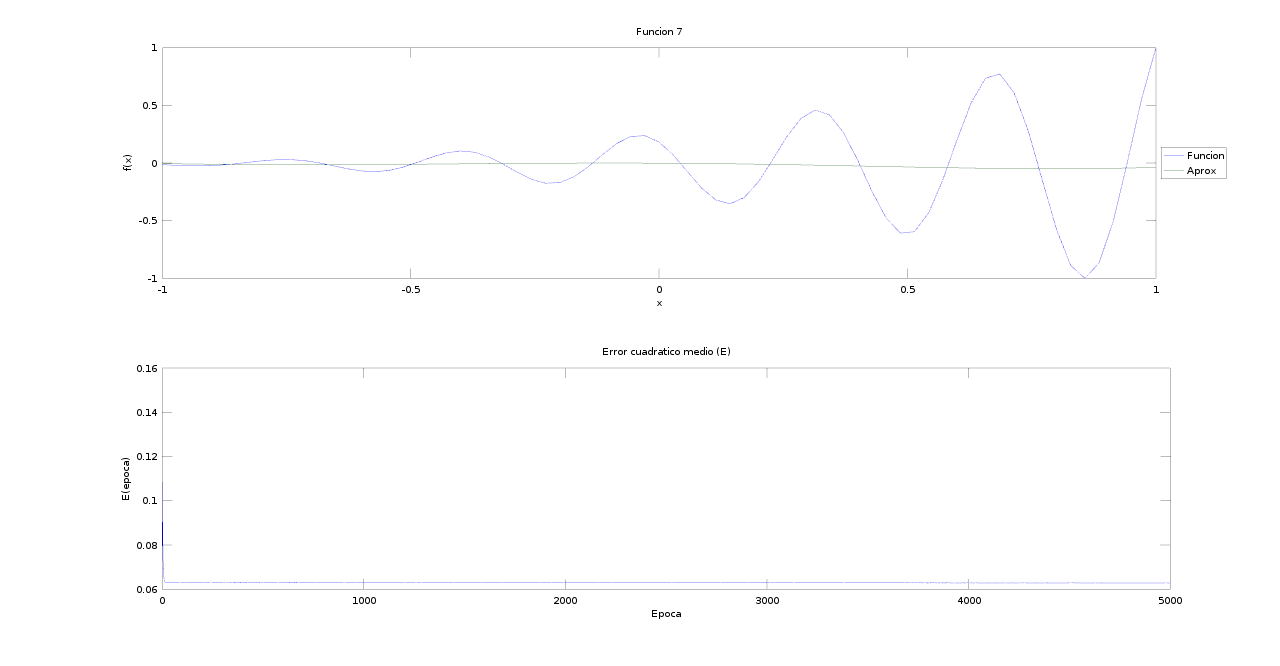
\includegraphics[width=0.85\textwidth]{img/PruebaRecu11.png}
\caption{\label{fig:PruebaRecu11} Prueba 1 de la tabla}
\end{figure}

\begin{figure}[h]
\centering
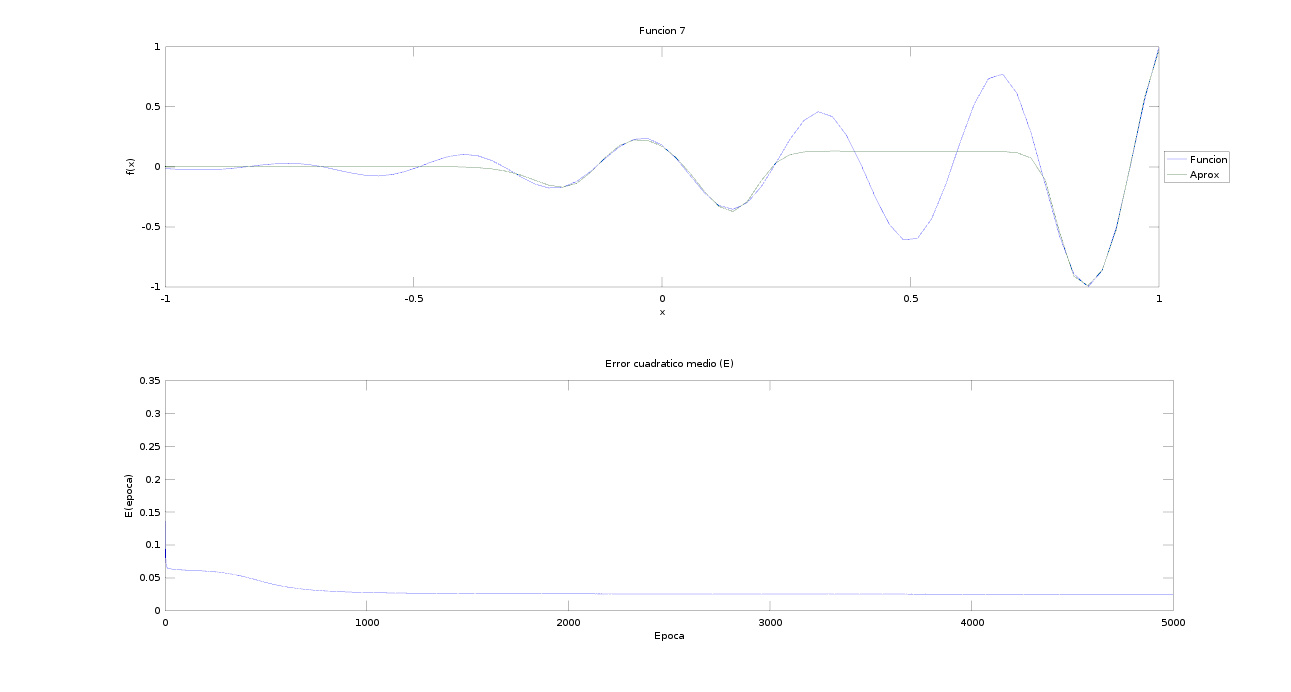
\includegraphics[width=0.85\textwidth]{img/PruebaRecu1.png}
\caption{\label{fig:pruebaRecu1} Prueba 1 de la tabla \ref{table:pruebaArqs}.}
\end{figure}

\begin{figure}[h]
\centering
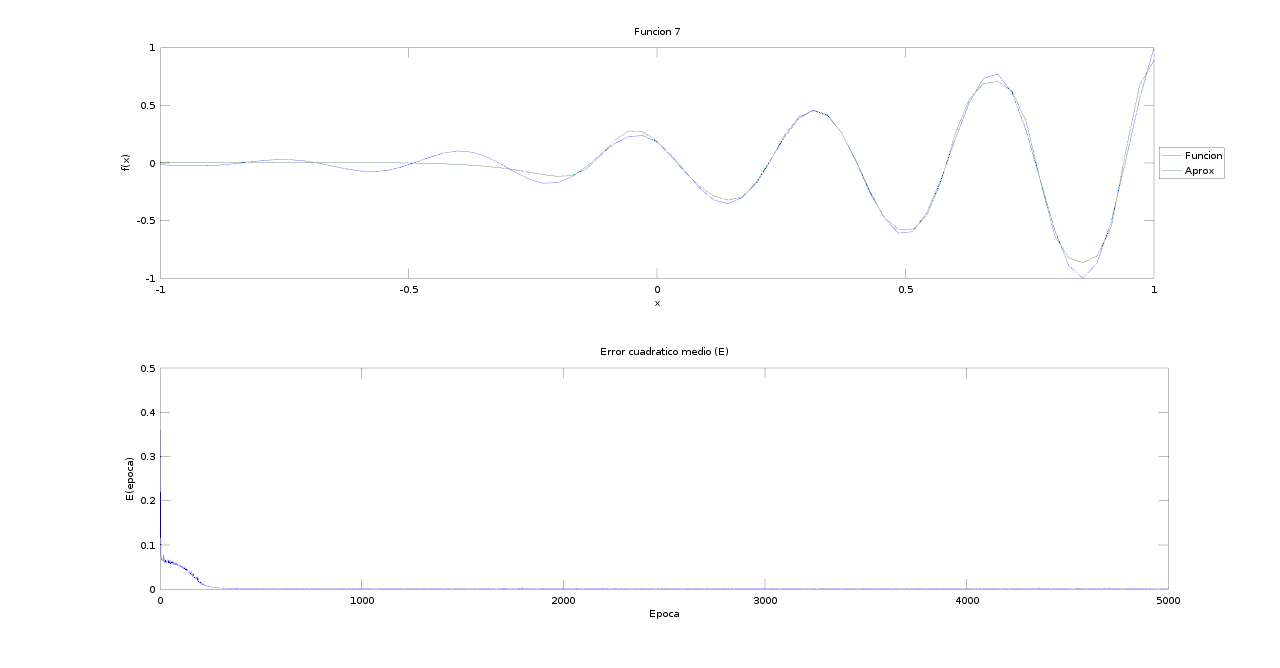
\includegraphics[width=0.85\textwidth]{img/PruebaRecu15.png}
\caption{\label{fig:pruebaRecu15} Prueba 2 de la tabla \ref{table:pruebaArqs}.}
\end{figure}

\begin{figure}[h]
\centering
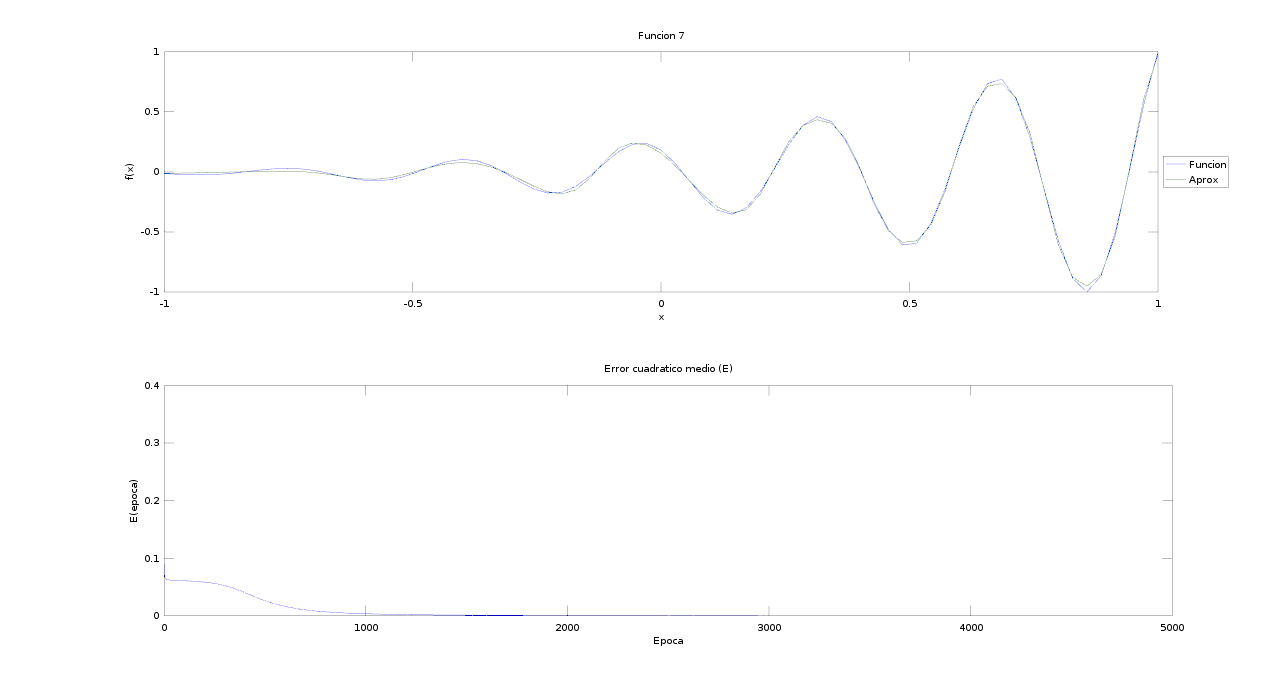
\includegraphics[width=0.85\textwidth]{img/PruebaRecu10.png}
\caption{\label{fig:pruebaRecu10} Prueba 5 de la tabla \ref{table:pruebaArqs}.}
\end{figure}


\end{document}